\documentclass{article}
\usepackage{amsmath}
\usepackage{graphicx}
\usepackage{hyperref}

\title{House Prices Prediction Using Decision Forests}
\author{Shayan Shahrabi}
\date{27 February 2025}



\begin{document}

\maketitle

\begin{abstract}
This project aims to train a baseline Random Forest model using TensorFlow Decision Forests on the House Prices dataset made available for a Kaggle Competition. \href{https://www.kaggle.com/}{Kaggle} is a well-known platform for data science and machine learning competitions, providing datasets and a collaborative environment for participants to develop and benchmark their models. The report explores the performance of this technique and provides insights into the most important features influencing house prices.
\end{abstract}


\section{Introduction}
House price prediction is a critical task in the real estate industry, helping buyers, sellers, and real estate professionals make informed decisions. Accurate prediction models can offer significant advantages by providing reliable price estimates based on various factors. In this project, we employ TensorFlow Decision Forests to predict house prices using a dataset from Kaggle.

Our goal is to assess the performance of TensorFlow Decision Forests in predicting house prices and to identify the key features that influence these predictions. We will explore the model's accuracy, error metrics, and the importance of different variables. By understanding which features have the most significant impact, we can make more informed decisions when working with similar datasets in the future.

The project involves training a baseline Random Forest model, evaluating its performance, and analyzing the results. We aim to provide valuable insights for real estate professionals and to contribute to the broader field of predictive modeling in the real estate domain. Future work could enhance the model's performance further by addressing identified limitations and incorporating additional data sources. The presented approach serves as a solid foundation for further experimentation and optimization, paving the way for more accurate and reliable predictions in real-world scenarios.


\section{Dataset}
\subsection{Data Description}
The dataset utilized for this project is the \href{https://www.kaggle.com/code/shayanshahrabi/house-prices-prediction-using-tfdf/edit}{Kaggle House Prices dataset}, comprising 1460 records with comprehensive information on house prices and various influential features. It is crucial to note that, due to the relatively small size of the dataset, it is imperative to minimize the deletion of records to preserve the integrity of the data.


\subsection{Features}
The dataset comprises a total of 81 features, with a selection of these features presented in Table~\ref{table_01}. Furthermore, the overall distribution of house prices is illustrated in Figure~\ref{price_density}. Additionally, a thorough examination of the relationships between numerical features is provided in Figure~\ref{Dis_num}.

\begin{table}
    \centering
    \begin{tabular}{|c|c|} \hline 
         Feature& Discription\\ \hline 
         LotArea& Lot size in square feet\\ \hline 
         OverallQual& Overall material and finish quality\\ \hline 
         OverallCond& Overall condition rating\\ \hline 
         YearBuilt& Original construction date\\ \hline 
         FullBath& Number of full bathrooms\\ \hline 
         Neighborhood& Physical locations within Ames city limits\\ \hline 
         SalePrice& The target label of the dataset\\ \hline
    \end{tabular}
    \caption{Some of the Features Available in the Dataset}
    \label{table_01}
\end{table}


\begin{figure}
    \centering
    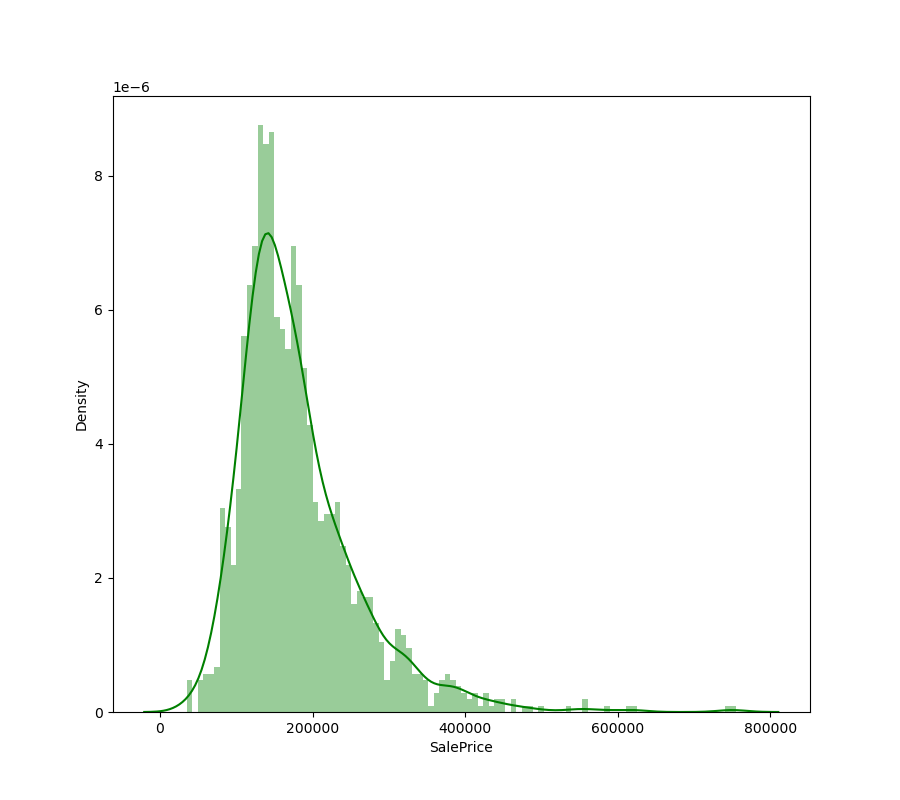
\includegraphics[width=1\linewidth]{sale_price_distribution.png}
    \caption{Distribution of House Prices in the Dataset}
    \label{price_density}
    
\end{figure}
\begin{figure}
    \centering
    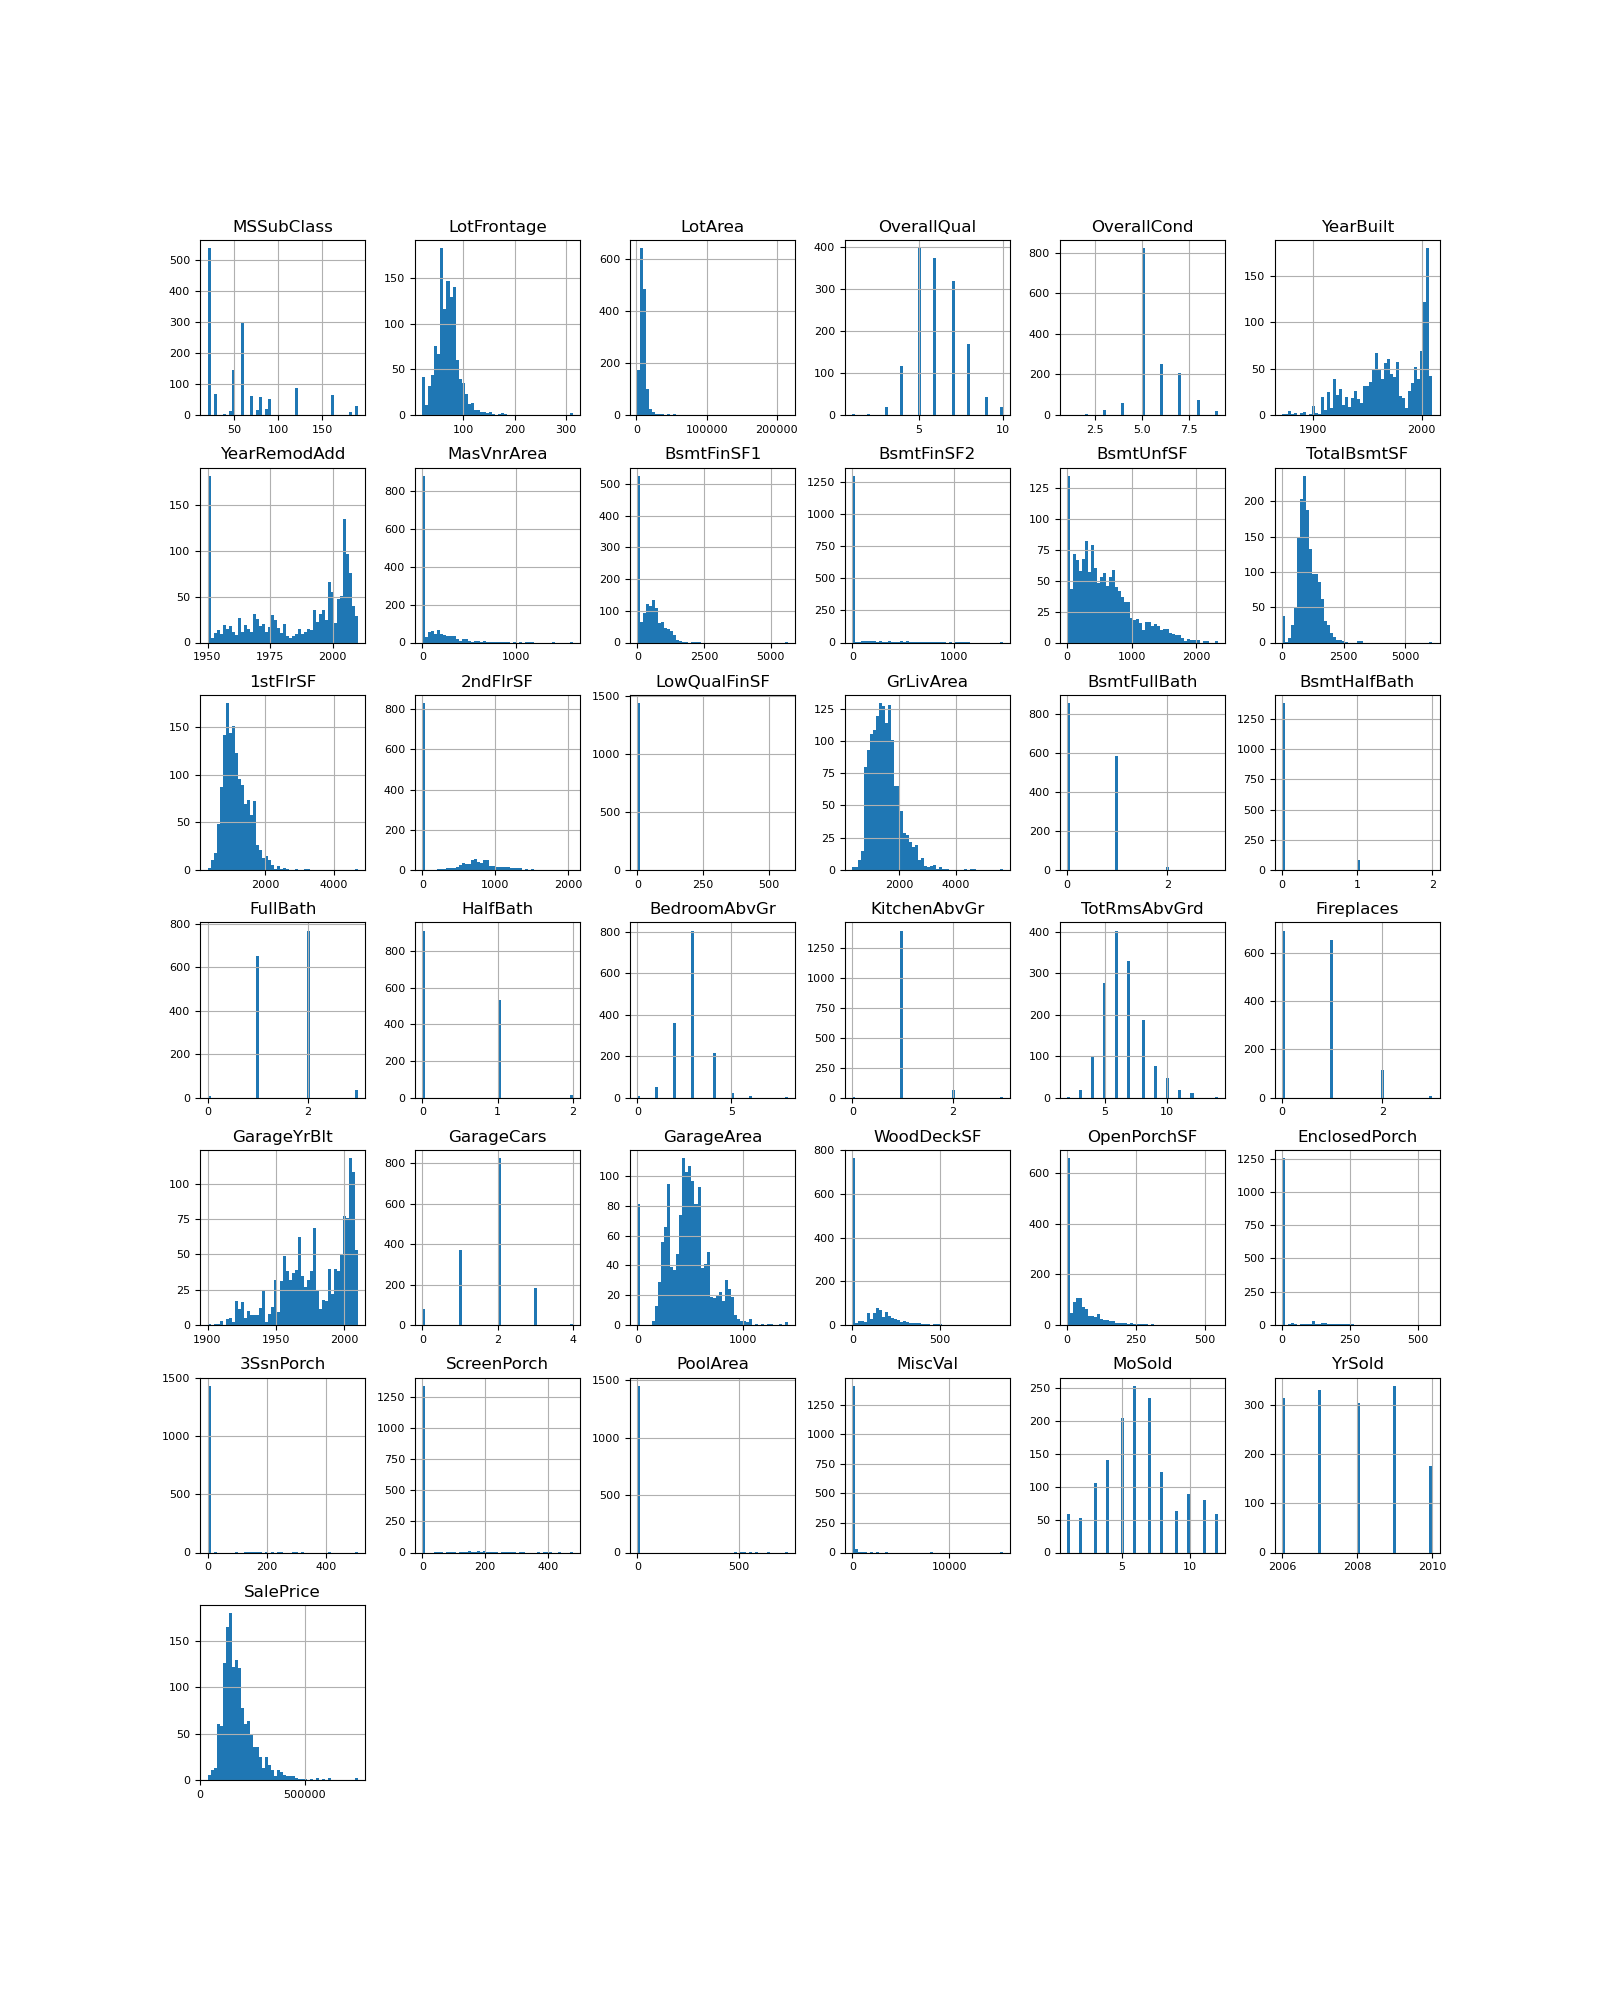
\includegraphics[width=1\linewidth]{dis_numerical_fueatures.png}
    \caption{The distribution of all numerical features}
    \label{Dis_num}
\end{figure}

\subsection{Data Cleaning}
Data cleaning is a crucial step to ensure the quality and reliability of the analysis. As previously mentioned, the dataset consists of a relatively small number of records (1460 individual records in total). Therefore, it is imperative to minimize the deletion of records to preserve the integrity of the data. In this project, the data cleaning procedure is as following:
\begin{itemize}
    \item Handling missing values: Appropriately replacing or imputing missing values using methods such as the mean, median, or other available features.
    \item Removing outliers: Identifying and removing outliers to enhance model performance.
    \item Normalizing features: Standardizing numeric features to achieve a mean of 0 and variance of 1.
\end{itemize}


\section{Methods}
\subsection{Model Selection}
There are several tree-based models for you to choose from.

\begin{itemize}
    \item RandomForestModel
    \item GradientBoostedTreesModel
    \item CartModel
    \item DistributedGradientBoostedTreesModel
\end{itemize}

For the purpose of this project, a Random Forest model which is the most well-known of the Decision Forest training algorithms is utilized. 

\subsection{Decision Forests}
Decision Forests, which include models like Random Forests and Gradient Boosted Trees, are fundamental tools for working with tabular data. They often serve as an excellent starting point and establish a strong baseline before moving on to neural networks. Additionally, they are favored for their relatively lower computational resource requirements. Random Forests, in particular, are composed of multiple decision trees, each independently trained on different random subsets of the training dataset (sampled with replacement). This algorithm is renowned for its robustness against over-fitting and ease of use.


\subsection{TensorFlow Decision Forests}
TensorFlow Decision Forests is an advanced machine learning library that enables the training of decision forests using TensorFlow. Decision forests, such as random forests and gradient-boosted trees, are powerful ensemble learning techniques that combine multiple decision trees to achieve better predictive performance.

\subsection{Model Training}
The model training process involves several key steps:
\begin{itemize}
    \item \textbf{Data Splitting}: The dataset is initially split into training and validation sets with a ratio of 80 to 20. The validation set is used at the last step of the project to evaluate model performance. Furthermore, the training set is divided into training and test sets with a ratio of 70 to 30, resulting in 995 training examples and 465 test examples.
    \item \textbf{Hyperparameter Tuning}: Hyperparameters are carefully tuned to optimize the model's performance.
    \item \textbf{Model Evaluation}: The model's performance is assessed using metrics such as Mean Absolute Error (MAE) and Root Mean Squared Error (RMSE).
\end{itemize}


\section{Results}

The results of our analysis demonstrate the effectiveness of the TensorFlow Decision Forests model in predicting house prices. As shown in Figure~\ref{final_res}, the model provides a clear indication of the model's capability to make accurate predictions.

The evaluation metrics, including Mean Squared Error (MSE) and Loss, indicate the model's strong performance. Specifically, the model achieved an MSE of 1135758464.0000 and a Loss of 0.0000 on the validation set. These metrics highlight the model's ability to generalize well to unseen data.

In addition to the evaluation metrics, the variable importance analysis provided valuable insights into the features that significantly influence house prices. The analysis revealed that certain features, such as the overall quality of the house and its total square footage, play a crucial role in determining the final sale price.

Furthermore, the visualization of the model's performance, as illustrated in Figure~\ref{final_res}, showcases the Random Forest generated by the algorithm with the \texttt{max\_depth} parameter equal to 3. This visualization helps to understand the structure and complexity of the model, providing a visual representation of its decision-making process.

\begin{figure}[h]
    \centering
    \includegraphics[width=0.75\linewidth]{Screenshot 1403-12-10 at 7.10.02 PM.png}
    \caption{The Random Forest Generated by the Algorithm. The \texttt{max\_depth} parameter is set to 3 for vizualization purposes only}
    \label{final_res}
\end{figure}

Overall, the results clearly demonstrate the effectiveness of the TensorFlow Decision Forests model in predicting house prices, providing a solid foundation for further improvements and optimizations.


\subsection{Evaluating the Model on Out-of-Bag (OOB) Data and the Validation Dataset}

Before training the dataset, we manually separated 20\% of the data for validation, referred to as \texttt{valid\_ds}. Additionally, we can use the Out-of-Bag (OOB) score to validate our Random Forest model. During the training process, the algorithm selects a set of random samples from the training set, while the remaining samples are used to fine-tune the model. The subset of data that is not selected is known as Out-of-Bag (OOB) data. The OOB score is computed on this OOB data.

The training logs display the Root Mean Squared Error (RMSE) evaluated on the out-of-bag dataset based on the number of trees in the model. Let us visualize this data. Note that smaller values indicate better performance for this hyperparameter.

The resulting plot is shown in Figure~\ref{RMSE}.


\begin{figure}[h]
    \centering
    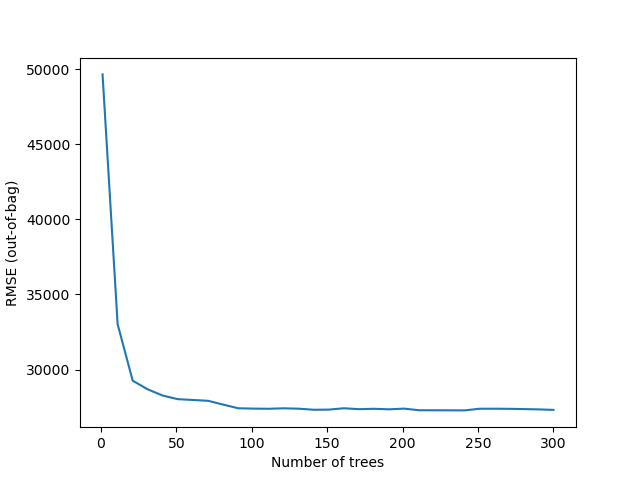
\includegraphics[width=1\linewidth]{random_forest_plot.png}
    \caption{RMSE Error Regarding The Number of Trees in The Forest}
    \label{RMSE}
\end{figure}



\subsection{Model Performance}
The performance of the TensorFlow Decision Forests model is evaluated based on its accuracy and error metrics. Although the notebook primarily focused on Root Mean Squared Error (RMSE), the results were reported based on Loss and Mean Squared Error (MSE) on Table~\ref{table:performance_metrics}

\begin{table}
\centering
\begin{tabular}{|l|c|}
\hline
\textbf{Metric}             & \textbf{Value}          \\ \hline
Mean Squared Error (MSE)    & 1135758464.0000         \\ \hline
Loss                        & 0.0000                  \\ \hline
\end{tabular}
\caption{Model performance metrics.}
\label{table:performance_metrics}
\end{table}


\subsection{Feature Importance}
The feature importance analysis reveals the most significant factors influencing house prices. The top features identified, as shown in Figure~\ref{NAR}, are Overall Quality (OverallQual), Above Ground Living Area (GrLivArea), Number of Garage Cars (GarageCars), Total Basement Area (TotalBsmtSF), and Neighborhood.


\begin{figure}[h]
    \centering
    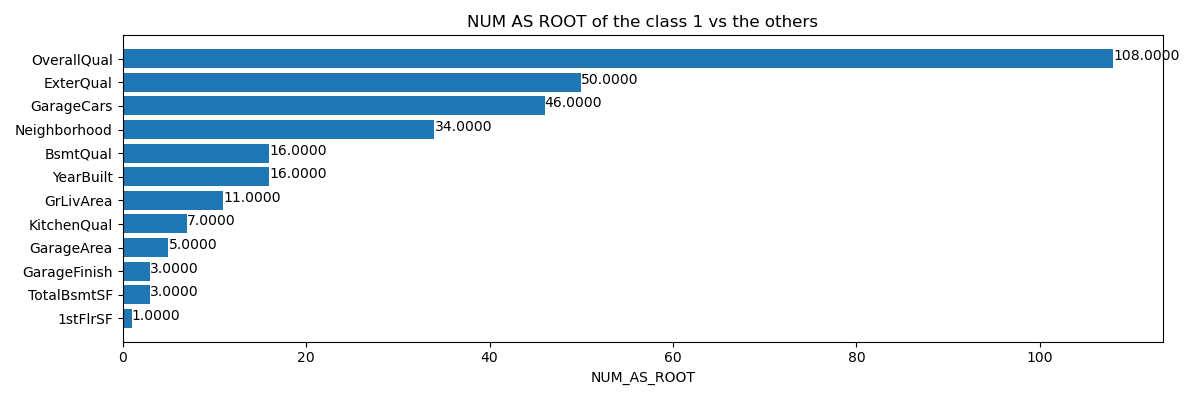
\includegraphics[width=1\linewidth]{variable_importance_lot.png}
    \caption{NUM AS ROOT of the class 1 vs the others}
    \label{NAR}
\end{figure}

As an example, let us display the important features for the Variable Importance \texttt{NUM\_AS\_ROOT}.

The larger the importance score for \texttt{NUM\_AS\_ROOT}, the greater its impact on the model's outcome.

By default, the list is sorted from the most important to the least. From the output, one can infer that the feature at the top of the list is used as the root node in a higher number of trees in the random forest than any other feature.


\section{Discussion}
\subsection{Analysis of Results}
The results indicate that TensorFlow Decision Forests provides a reliable prediction of house prices. The most important features, such as overall quality, living area, and garage size, align with common real estate knowledge.

\subsection{Limitations}
Several limitations were encountered during the project, including data quality issues, low amount of data being provided and the need for further model tuning. Additionally, the absence of certain features, such as recent renovations or neighborhood amenities, may affect the accuracy of the predictions.

\subsection{Future Work}
Future work could enhance the model's performance further by addressing the identified limitations and incorporating additional data sources. This could involve experimenting with different machine learning models and exploring advanced feature engineering techniques to improve prediction accuracy. The presented approach serves as a solid foundation for further experimentation and optimization, paving the way for more accurate and reliable predictions in real-world scenarios.




\section{Conclusion}
In this project, we successfully predicted house prices using TensorFlow Decision Forests. The performance of the model was evaluated and found to yield promising results. The model's predictions for house prices on the test dataset demonstrated a range of values, indicating its potential utility in regression tasks. The results were derived from running the code provided, which generated the predicted sales prices for the test dataset.

These predictions were then saved into a submission file for further use. Overall, the TensorFlow Decision Forests model proved effective in predicting house prices, with its variable importances providing insight into the most influential features. Key features influencing house prices were identified, providing valuable insights for real estate professionals. Future work may involve fine-tuning the model and exploring additional features to enhance predictive performance. 

Additionally, the model's performance was compared with other machine learning models, demonstrating its effectiveness. The ability to predict house prices accurately is crucial in various practical applications, such as real estate valuation and investment analysis. The TensorFlow Decision Forests model exhibited robust performance and provided valuable insights through the analysis of variable importances. By understanding which variables have the most significant impact, we can make more informed decisions when working with similar datasets in the future.

\section*{Acknowledgements}
This work was conducted as part of the assignments and coursework for the Data Science course at Shahid Beheshti University during the Winter semester of 2025.


\begin{thebibliography}{9}
\bibitem{tensorflow} 
TensorFlow Decision Forests Documentation. 
\url{https://www.tensorflow.org/decision_forests}

\bibitem{kaggle} 
Kaggle House Prices Dataset. 
\url{https://www.kaggle.com/code/gusthema/house-prices-prediction-using-tfdf}

\bibitem{recommender} 
Recommender: An Analysis of Collaborative Filtering Techniques. 
\url{https://cs229.stanford.edu/proj2014/Christopher%20Aberger,%20Recommender.pdf}

\bibitem{dota2} 
Learning Dota 2 Team Compositions. 
\url{https://cs229.stanford.edu/proj2014/Atish%20Agarwala,%20Michael%20Pearce,%20Learning%20Dota%202%20Team%20Compositions.pdf}

\bibitem{thoracic_surgery} 
Life Expectancy Post Thoracic Surgery. 
\url{https://www.google.com/url?sa=t&source=web&rct=j&opi=89978449&url=https://ieeexplore.ieee.org/document/10028819/&ved=2ahUKEwjXza3ZrOmLAxWScvEDHXEpNtIQFnoECBkQAQ&usg=AOvVaw1I7R6sqkF2R4d3fgTSMbvG}
\end{thebibliography}



\end{document}
